\documentclass[11pt]{beamer}
\usepackage[utf8]{inputenc}
\usecolortheme{beaver}
\usepackage{graphicx}
\setbeamercolor{itemize item}{fg=darkred!80!black}
\setbeamertemplate{navigation symbols}{}%remove navigation symbols

%Information to be included in the title page:
\title{Containers, Kube, OH MY!}

\graphicspath{ {../assets/files} }

\begin{document}

\frame{\titlepage}

\begin{frame}
  \frametitle{Who Am I?}
  Hi I'm Tim Olson
  \begin{itemize}
    \item Site Reliability Engineer
    \item Kubestuff since 2017
    \item Linux fanatic
  \end{itemize}
\end{frame}

\begin{frame}
  \frametitle{Guidelines}
  \begin{itemize}
    \item If you have a question, others might too.
    \begin{itemize}
      \item I'm long winded. Interrupt me!
      \item I'll try to keep an eye on chat.
      \item I will have a recording.
    \end{itemize}
    \item There is no gate keeping here. Welcome!
    \item Following the lecture. PLEASE reach out for any assistance.
  \end{itemize}
\end{frame}

\begin{frame}
  \frametitle{History}
  \begin{itemize}

  \item (1950) In the beginning there were mainframes.
  \item (1971) Along comes UNIX a multiuser, multitasking operating system!
  \begin{itemize}
    \item Running concurrent jobs is now much easier!
    \item Time begins _for real_.
  \end{itemize}
  \item (1991) Linux released
  \item (2000) FreeBSD jails
  \begin{itemize}
    \item Environmental virtualization
    \item Each jail is isolated from a security perspective
  \end{itemize}
  \item (2003) Xen is released, the first open-source x86 hypervisor
  \begin{itemize}
    \item AWS currently runs on top of Xen and is moving to KVM (2007)
  \end{itemize}
  \item (2013) Docker released\*
  \item (2014) Kubernetes released\*
  \item (2015) Cloud Native Computing Foundation founded.
  \item (2015) containerd, (2014) runc, kubernetes, (2012) prometheus, etc
  \end{itemize}
\end{frame}

\begin{frame}
  \frametitle{Example monolith from 2000s}
  Traditional deploys often followed monolithic architecture. Or maybe just me in 2007...

  LAMP Stack
  \begin{itemize}
    \item Linux - The operating system it all runs on.
    \item Apache - The weberver to host assets
    \item MySQL - The database for the application
    \item PHP - Server side scripting language, what the client sees.
  \end{itemize}
\end{frame}

\begin{frame}
  \begin{center}
    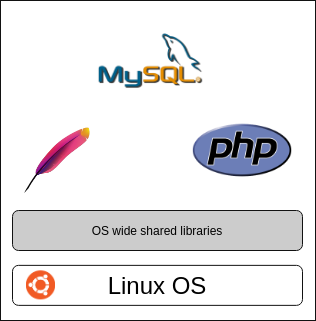
\includegraphics[width=120px,keepaspectratio]{LAMP}
  \end{center}
\end{frame}

\begin{frame}
  \frametitle{Example monolith from 2000s}
  Traditional deploys often followed monolithic architecture. Or maybe just me in 2007...

  How might we deploy or operate this?
  \begin{itemize}
    \item Ubuntu linux host, tools installed locally.
    \begin{itemize}
      \item `apt install php7.4 php7.4-mysql apache2 mariadb`
    \end{itemize}
    \item Source code is in git
    \item Deployment operates by ansible - logs into the box, pulls new git main branch
    \item What problems might we face with this?
  \end{itemize}
  Before we leave, let's not blame this on the individual components, and treat containers like
  they solve all the problems. Let's just recognize some of the characteristics of containers
  that might benefit our architecture design.

\end{frame}

\begin{frame}
  \begin{center}
    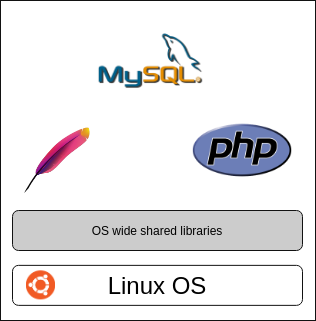
\includegraphics[width=120px,keepaspectratio]{LAMP}
  \end{center}
\end{frame}

\begin{frame}
  \begin{center}
    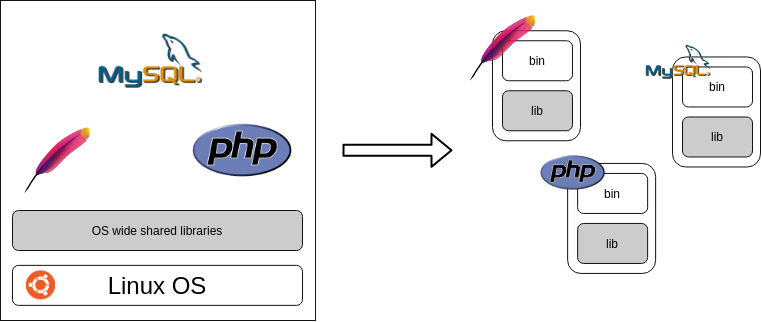
\includegraphics[width=280px,keepaspectratio]{BNW}
  \end{center}
\end{frame}

\begin{frame}
  \begin{center}
    Containers
  \end{center}
\end{frame}

\begin{frame}
  \frametitle{Containers}
  What is a container?:
  \begin{itemize}
    \item An execution environment running a process, which is derived from a container image.
  \end{itemize}
  Ok so what's an image?
  \begin{itemize}
    \item An ordered collection of union file systems, which makes up execution parameters for a process, and includes companion binaries and libraries.
  \end{itemize}
\end{frame}

\begin{frame}
  \frametitle{Containers}
  Two major pices of kernel tech that help us get this done:
  \begin{itemize}
    \item cgroups
    \item namespaces
    \begin{itemize}
      \item `pid` - Responsible for process isolation
      \item `net` - manages network isolation
      \item `ipc` - manages inter process communication
      \item `mnt` - manages filesystem mounts
      \item `uts` - manages kernel isolation and version identifiers (derived rom Unix Time-Sharing System)
      \item `usr` - manages uid isolation
      \item `cgroup` - manages control group info from container
    \end{itemize}
  \end{itemize}
\end{frame}

\begin{frame}
  \begin{center}
    drop to a shell
  \end{center}
\end{frame}

\begin{frame}
  \begin{center}
    Host does this compare to a VM?
  \end{center}
  \begin{center}
    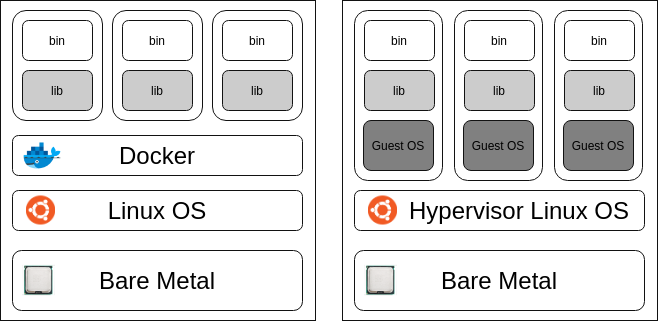
\includegraphics[width=220px,keepaspectratio]{dockerVM}
  \end{center}
  \begin{center}
    This can get funky. Technically the left picture can also be the Guest OS/lib/bin block too!
  \end{center}
\end{frame}

\begin{frame}
  \frametitle{Containers}
  What components make up an Operating System?
  \begin{enumerate}
    \item Has an Init System
    \item Has it's own Kernel
    \item Likely runs multiple services, e.g.
    \begin{itemize}
      \item Networking
      \item User system
      \item Network time service
    \end{itemize}
   \item Might have GUI or other sys admin tools onboard
  \end{enumerate}
  drop to a shell
\end{frame}

\begin{frame}
  \begin{center}
    Time to look at the docker development with the CLI!
  \end{center}
\end{frame}

\begin{frame}
  \frametitle{Containers}
    Let's recap some things about docker development
  \begin{itemize}
    \item What two core things make a docker container work?
    \item Difference between a container and an image
    \item How do we build images, what is a union file system
    \item How are the parent images made and how can we see how they work
    \item Handy things with docker?; entrypoints, development tooling
  \end{itemize}
\end{frame}

\begin{frame}
  \begin{center}
    Kuberentes
  \end{center}
\end{frame}

\begin{frame}
  \frametitle{Kubernetes}
    To me "It's just a scheduler"
  \begin{itemize}
    \item "The responsibility of the control loop is to constantly audit the desired state of the cluster to the current state of the cluster."
  \end{itemize}
    Kubernetes is a platform to run containers at scale!
  \begin{itemize}
    \item We get an ecoystem of turnkey monitoring, logging, autoscaling, service discovery, and so much more.
  \end{itemize}
\end{frame}

\begin{frame}
  \begin{center}
    Kube architecture
  \end{center}
  \begin{center}
    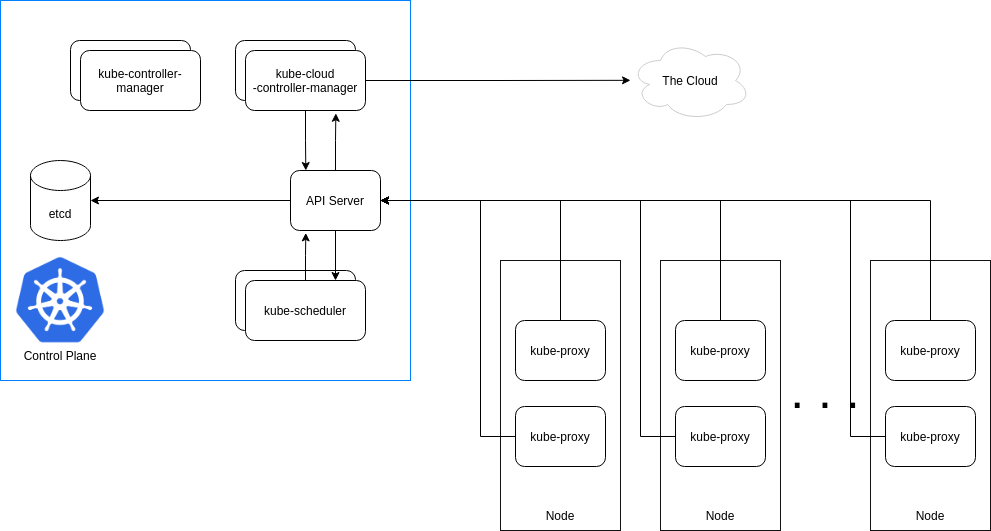
\includegraphics[width=220px,keepaspectratio]{control-plane}
  \end{center}
\end{frame}

\end{document}
